%!TEX root = ../thesis.tex

\vspace{-10pt}

\section{本章の概要}
本章では,\ref{sec:nav-sys}節でシステムの概要を示す.また,\ref{sec:real-robot}節で実ロボットにおける歩行者の位置計算の詳細,\ref{sec:nav-usage}節でナビゲーションにおける予測結果の利用方法について述べる.

% \newpage

\section{システム概要}\label{sec:nav-sys}
\figref{Fig:nav-system}に,ナビゲーションシステムの概要図を示す.主に構成しているモジュールを以下に示す.

\begin{itemize}
  \item \textbf{制御モジュール} \\
  制御モジュールは,Navigation Stackの主要コンポーネントであるmove\_baseで構成されている.
  センサデータと目標位置を受け取り,適切なロボットの制御指令を出力する.
  \item \textbf{認識モジュール} \\
  認識モジュールは,YOLOを用いて歩行者の検出及び,追跡を行う.そして,観測時間分のデータをまとめて時系列データとして出力する.
  \item \textbf{予測モジュール} \\
  予測モジュールは,認識モジュールからメッセージを受け取り,そのデータを基に\ref{chap:proposed_method}章で述べたネットワークを用いて歩行者の位置予測を行う.その後,制御モジュールのglobal\_costmapの独自レイヤで予測結果をコストマップに反映する.
\end{itemize}

\newpage

\vspace*{15pt}

\begin{figure}[H]
  \centering
 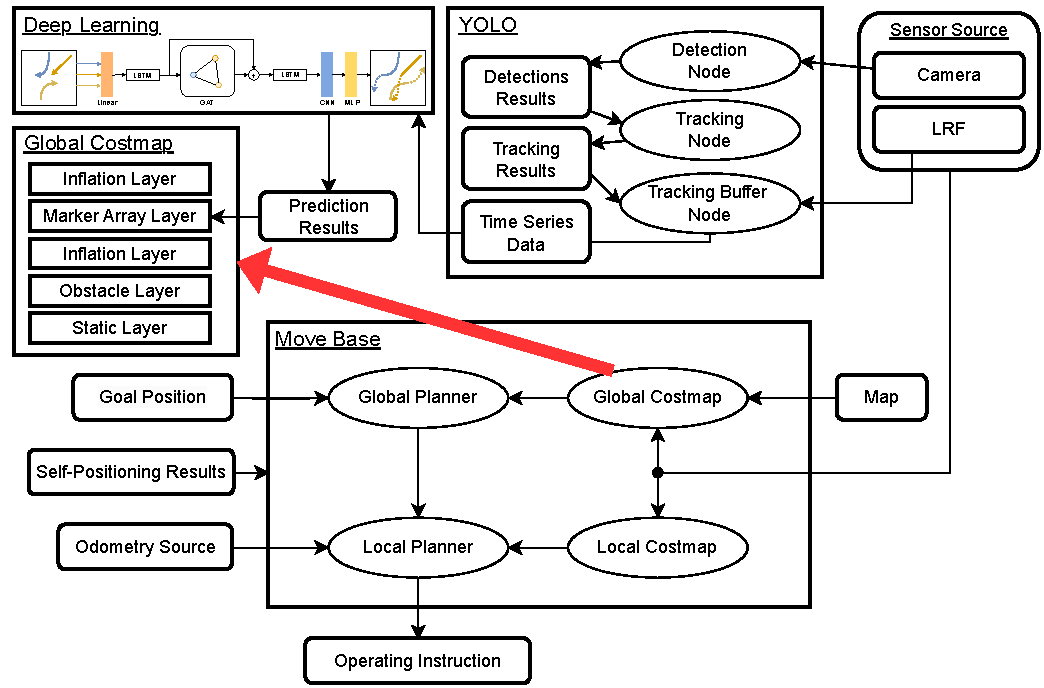
\includegraphics[keepaspectratio, scale=0.77]
      {images/application_system.pdf}
 \caption{Navigation System Overview}
 \label{Fig:nav-system}
\end{figure}  

\section{実ロボットにおける歩行者の位置計算}\label{sec:real-robot}
データセットと実ロボットにおける歩行者の位置計算のイメージを\figref{Fig:ped2pos}に示す.ここで,データセットはETH\cite{pellegrini2009you-eth},UCY\cite{lerner2007crowds-ucy}データセットのような,俯瞰視点のデータセットのことを指す.\figref{Fig:ped2pos-dataset}のように,データセットでは,俯瞰視点の映像と各時刻における歩行者のワールド座標系上の位置が含まれている.しかし,実ロボットではセンシングしたデータのみで,ワールド座標系の位置計算が求められる.一例として\figref{Fig:ped2pos-realrobot}のように,1人称視点の画像上の歩行者の位置を,ワールド座標系での位置に座標変換し,データセットとデータ形式を合わせる必要がある.そうすることで,データセットで学習した訓練済みモデルを実ロボットにおいても再学習することなく,そのまま利用することができる.

\begin{figure}[H]
  \centering
  \begin{minipage}{0.85\textwidth}
    \centering
    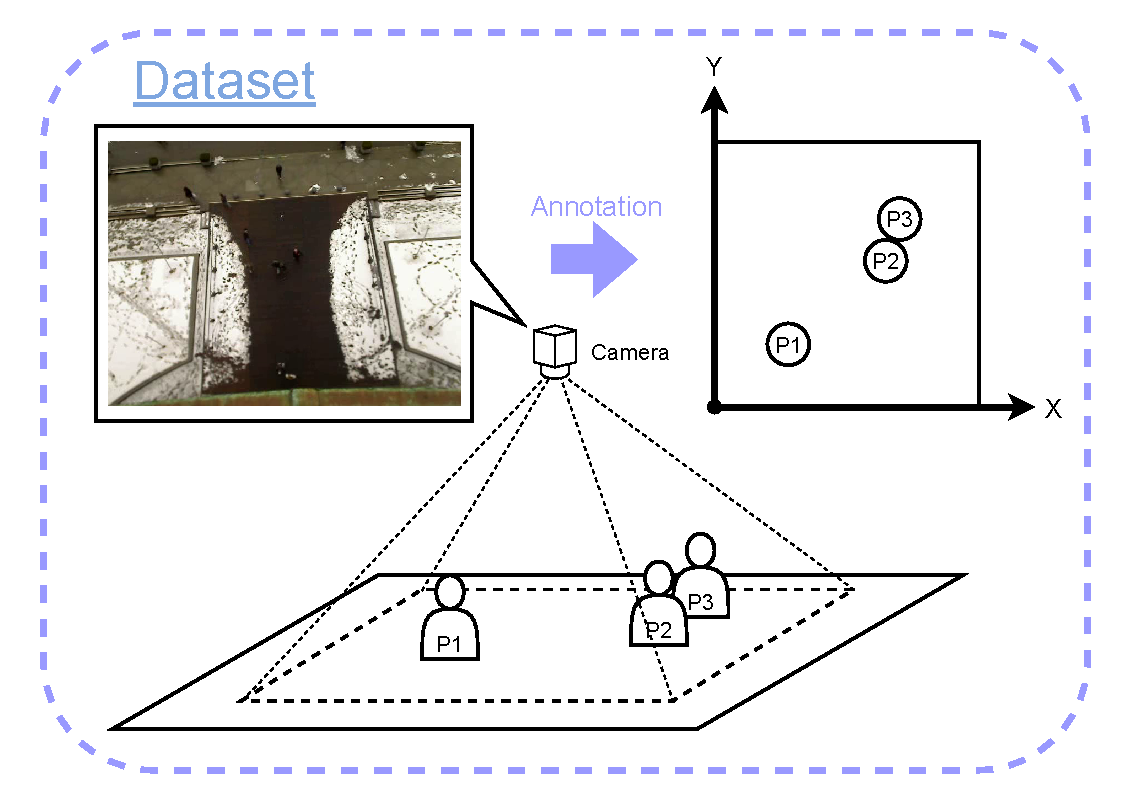
\includegraphics[width=\linewidth]{images/ped2pos-dataset.pdf}
    \subcaption{Pedestrian Position Calculation on Dataset}
    \label{Fig:ped2pos-dataset}
  \end{minipage}
  \hfill
  \begin{minipage}{0.85\textwidth}
    \centering
    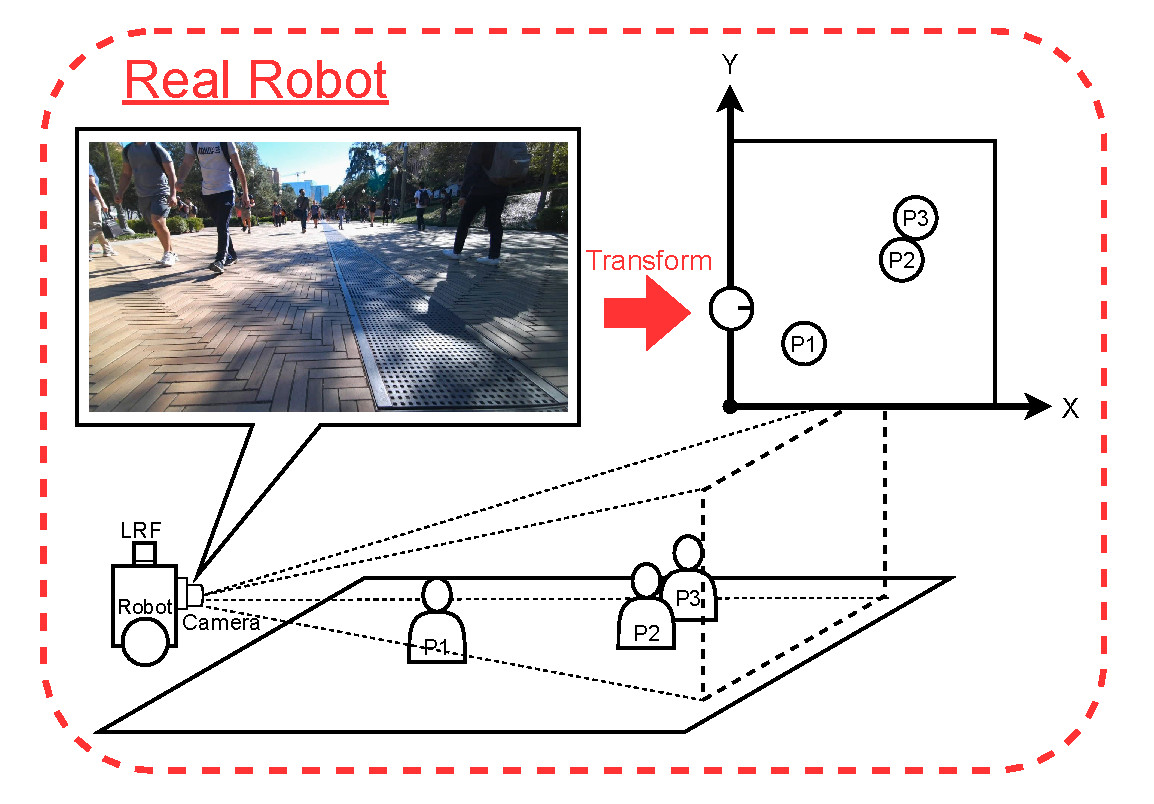
\includegraphics[width=\linewidth]{images/ped2pos-realrobot.pdf}
    \subcaption{Pedestrian Position Calculation on Real Robot}
    \label{Fig:ped2pos-realrobot}
  \end{minipage}
  \caption{Pedestrian Position Calculation: (a) on Dataset, (b) on Real Robot}
  \label{Fig:ped2pos}
\end{figure}
% \protect\footnotetext[8]{\cite{pellegrini2009you-eth}より画像を引用}
% \protect\footnotetext[9]{\cite{karnan2022socially-scand}より画像を引用}

\newpage

以下に,本研究での実ロボットにおける歩行者の位置計算の流れと詳細を示す.
% その後,各処理の詳細について述べる.
% \begin{enumerate}
%   \item RGBカメラ画像とLRFデータを取得
%   \item YOLOで人間検出
%   \item 検出した個体の画像上での角度を計算
%   \item 計算した角度とLRFデータからロボットとの相対位置を計算
%   \item 相対位置をワールド座標へ座標変換
% \end{enumerate}

\begin{enumerate}
  \item \textbf{RGBカメラ画像とLRFデータを取得} \\
  RGBカメラは,ロボットの前方に取り付けられており,歩行者の画像を取得する.また,LRF(Laser Range Finder)は,ロボットの周囲の距離データを取得するために使用される.これらのデータは,歩行者の位置推定に必要な情報を提供する.

  \item \textbf{YOLOで人間検出} \\
  YOLO\cite{redmon2016you-yolo}は,リアルタイム物体検出アルゴリズムであり,RGBカメラ画像から歩行者を検出するために使用される.YOLOは,高速かつ高精度な検出が可能であり,歩行者の位置を画像上で特定する.本研究では,YOLOv9\cite{wang2025yolov9}の学習済みモデルを用いる.

  \item \textbf{検出した個体の画像上での角度を計算} \\
  検出された歩行者の位置を基に,画像上での角度を計算する.この角度は,ロボットのカメラの視野内での歩行者の位置を示す.計算式を以下の式\eqref{yolo-ang}に示す.

  \begin{equation}
    \theta_{camera} = - \cfrac{(x_{center} - \cfrac{w_{img}}{2}) \cdot fov_{horizontal}}{W_{img}} \label{yolo-ang}
  \end{equation}

  なお,$w_{img}$は画像の幅,$fov_{horizontal}$は水平視野角,$x_{center}$が検出した物体のバウンディングボックスの中心$x$座標である.計算後,$\theta_{camera}$を$-\pi \text{から} \pi$の範囲に正規化する.

  \item \textbf{計算した角度とLRFデータからロボットとの相対位置を計算} \\
  画像上で計算された角度を基に,LRFデータの対応する角度の要素を取り出す.そして,そのデータを用いて歩行者とロボットとの相対位置を計算する.LRFデータは,ロボットからの距離情報を提供し,歩行者の正確な位置を特定するために使用される.

  \item \textbf{相対位置をワールド座標へ座標変換} \\
  最後に,計算された相対位置をワールド座標系に変換する.この座標変換は,ロボットのナビゲーションシステムのmapフレームに基づいて行われる.ワールド座標系での位置が特定されることで,ロボットは歩行者の位置を正確に把握し,適切なナビゲーションを行うことができる.
\end{enumerate}

\section{ナビゲーションにおける予測結果の利用方法}\label{sec:nav-usage}
\figref{Fig:global-costmap}に示すように,グローバルコストマップに独自のレイヤであるMarker Array Layerを追加した.このレイヤでは,予測結果を受け取るたびにコストマップに反映する.なお,予測結果は0.4秒ごとに受け取る.
\ref{sec:decoder}節で述べたように,予測結果のデータ形式はガウス分布を構成する5次元の要素である.本研究では,そのガウス分布からサンプリングした軌道を予測結果として,コストマップに反映する.
\figref{Fig:costmap-flow}のように,各レイヤでの処理を積み重ねて,最終的なグローバルコストマップを生成する.グローバルコストマップを拡張したのは,\ref{sec:navigation-stack}項で述べたように,多くのロボットで使用されているNavigation Stackで予測結果を容易に利用できるようにするためである.

\begin{figure}[H]
  \centering
 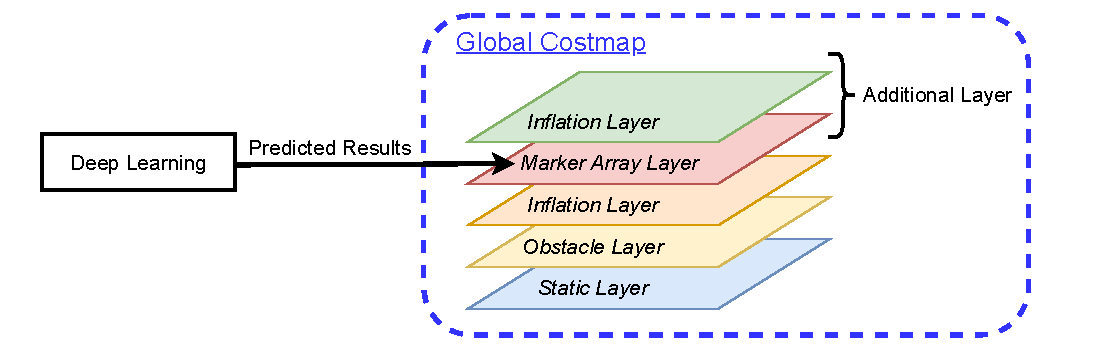
\includegraphics[keepaspectratio, scale=0.7]
      {images/layer.pdf}
\caption{Global Costmap in This Study}
 \label{Fig:global-costmap}
\end{figure} 

\begin{figure}[H]
  \centering
 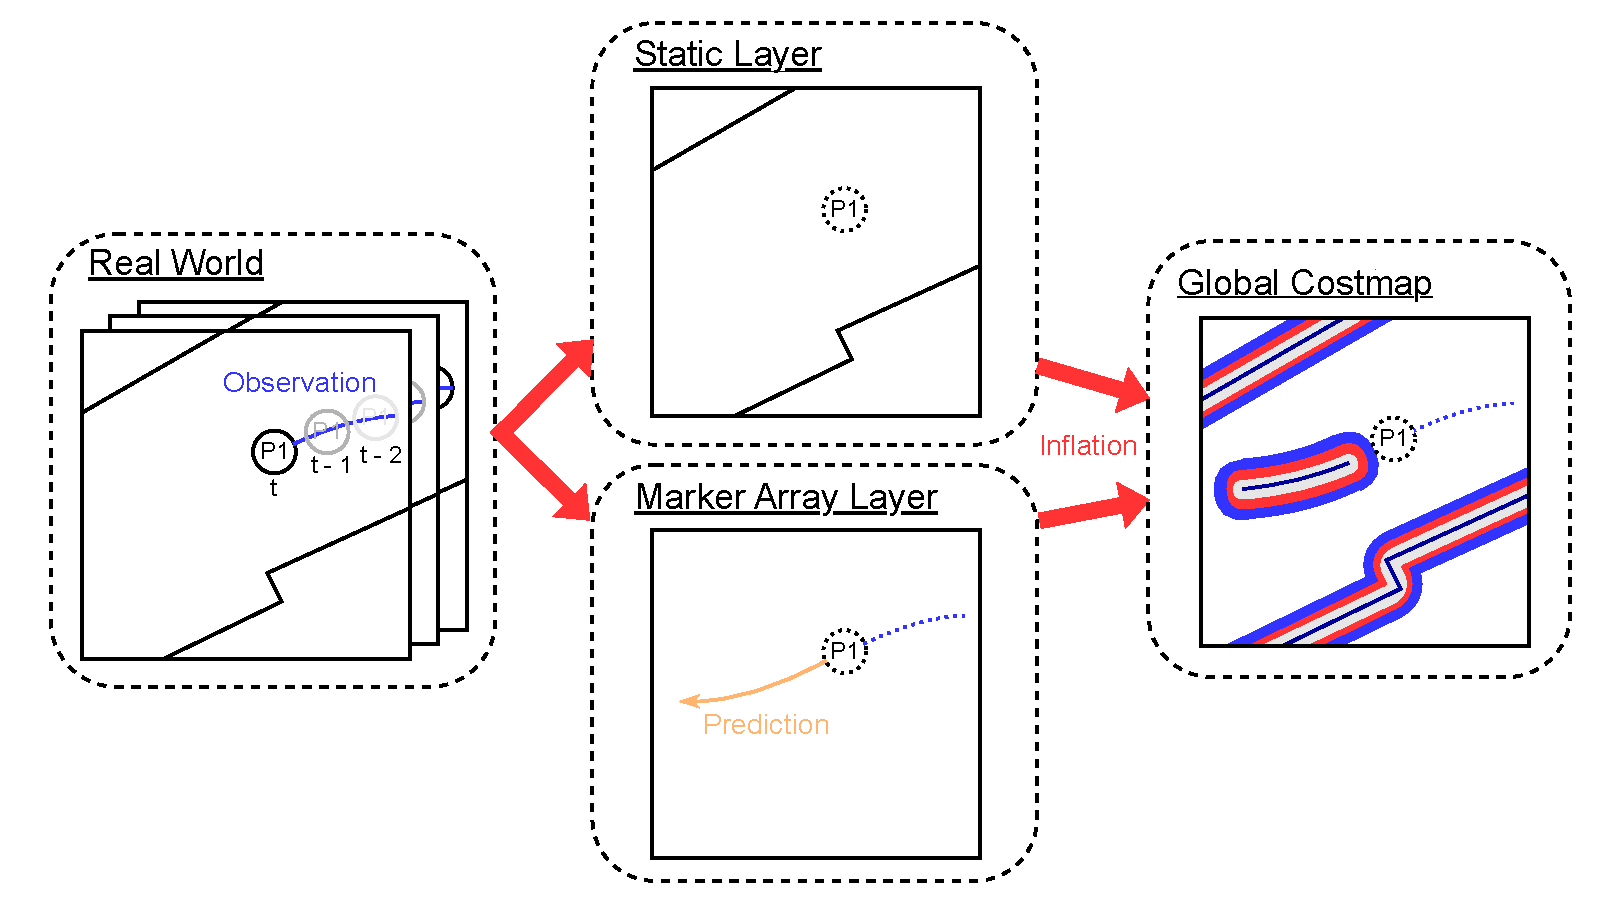
\includegraphics[keepaspectratio, scale=0.47]
      {images/costmap-image.pdf}
\caption{Process each layer to generate a global costmap}
 \label{Fig:costmap-flow}
\end{figure} 


\newpage
